% vim: set textwidth=78 autoindent:

\subsection{Plugin di Cattura delle Coordinate}

% when the revision of a section has been finalized, 
% comment out the following line:
% \updatedisclaimer

Il plugin di Cattura delle Coordinate è facile da usare e offre la capacità di mostrare sulla mappa le coordinate per due Sistemi di Riferimento tramite Coordinate (Coordinate Reference Systems - CRS). Basta cliccare un certo punto e copiare le coordinate negli appunti o usare la funzionalità di tracciatura del mouse.

\begin{figure}[ht]
   \begin{center}
   \caption{Plugin di cattura delle Coordinate\nixcaption}\label{fig:coordinate_capture_dialog}\smallskip
   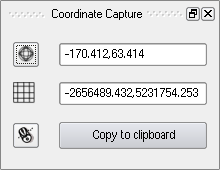
\includegraphics[clip=true]{coordinate_capture_dialog}
\end{center}  
\end{figure}

\begin{enumerate}
  \item Lanciare QGIS, selezionare \dropmenuopttwo{mActionOptions}{Proprietà Progetto} dal menu
  \mainmenuopt{Impostazioni} e scegliere la tab \tab{Sistema Riferimento Spaziale (SRS)}. In alternativa, cliccare l'icona \toolbtntwo{mIconProjectionEnabled}{Stato SRS} nell'angolo in basso a destra della barra di stato.
  \item Selezionare \checkbox{Abilita la modifica immediata SRS Information} 
  \filename{"NAD27/Alaska Albers"} con EPSG 2964 (vedi anche la Sezione \ref{label_projections}).
  \item Caricare il layer vettoriale \filename{alaska.shp} dal set di dati campione QGIS.
  \item Caricare il plugin di Cattura di Coordinate nel Gestore dei Plugins (vedere la Sezione 
  \ref{sec:load_core_plugin}) e selezionare l'icona \toolbtntwo{coordinate_capture}{Cattura delle Coordinate}. Compare una finestra di dialogo della Cattura di Coordinate come mostrato in Figura \ref{fig:coordinate_capture_dialog}.
  \item Selezionare l'icona \toolbtntwo{geographic}{Clicca per selezionare il SRS da usare durante la visualizzazione delle coordinate}, espandere la lista Sistemi di Coordinate Geografiche e scegliere \filename{WGS84} (EPSG 4326).
  \item Ora si può cliccare ovunque sulla mappa e il plugin mostrerà le coordinate 
  \filename{"NAD27/Alaska Albers"} e \filename{WGS84} per il punto selezionato come mostrato nella Figura \ref{fig:coordinate_capture_dialog}.
  \item Per abilitare la tracciatura mouse delle coordinate selezionare l'icona \toolbtntwo{tracking}{tracciatura mouse}.
  \item Si possono anche copiare le coordinate selezionate negli appunti.
\end{enumerate}

\newpage



